\mychapter{Credential Relationship Binding Nullifier}

\section{Problem Statement and Motivation}
Anonymous Credential systems must balance user privacy with protection against Sybil attacks, where a malicious user creates multiple credentials. In our $\MIMCABC$ based Identity System, users possess a Master Credential containing a secret key $\k$ and may obtain multiple Context Credentials for different services or contexts. Each Context Credential contains a unique identifier $\ctx$ (e.g., $\mathcal{H}(\text{``DriverLicense''})$). During issuance, the system must ensure that each user receives at most one credential per context—without compromising privacy by revealing user identities.

Specifically, we need a privacy-preserving mechanism we need that creates a unique deterministic token (nullifier) for each user-context pair without compromising anonymity.

\subsection{Limitations of Existing Approaches}

Verifiable Random Functions (VRFs) offer a promising foundation for nullifier construction, but existing implementations have significant limitations:

\begin{itemize}
    \item \textbf{Standard VRF:} Traditional constructions expose the user's public key during verification, breaking unlinkability between credential uses~\cite{hutchison_verifiable_2005}

    \item \textbf{MPC PRF} Systems like CanDID~\cite{maram2021candid} use secure multi-party computation to preserve anonymity but introduce substantial overhead and prevent dynamic nullifier generation.

    \item \textbf{Pairing-based Approaches:} Recent constructions like UTT~\cite{tomescu2022utt} use bilinear pairings and committed attributes that, while secure, are computationally expensive—often 5-10× slower than standard group operations.
\end{itemize}

Our approach introduces a pairing-free nullifier construction optimized for anonymous credentials, providing strong privacy guarantees with practical efficiency.


\subsection{Contributions}

\noindent We improve the state of the art by creating a lightweight VRF construction tailored for Anonymous Credential systems with 3 contributions:
\begin{enumerate}
        \item \textbf{Pairing-Free VRF in Prime-Order Groups:} We adapt the Dodis-Yampolskiy VRF structure to function efficiently in standard prime-order groups, achieving provable pseudorandomness under the $q$-Diffie-Hellman Inversion ($q$-DHI) assumption. We show that VRF evaluation is 33\% faster and verification is 60\% faster than previous constructions.

        \item \textbf{Zero-Knowledge Proof of Multiplicative Inverse:} We introduce a novel $\Sigma$-protocol that proves the multiplicative inverse relation between committed values $(\k + \ctx)$ and $1/(\k + \ctx)$, we use it in our scheme to verify the correctness of the VRF nullifier without revealing user secrets. We show it generalizes naturally for similar requirements in $\Sigma$-protocols, especially those needing to prove the q-DHI.

         \item \textbf{Formal Security Guarantees:} maintains \emph{Pseudorandomness} of the VRF outputs in the indistinguishable outputs, \emph{uniqueness} in one nullifier per $(k, \ctx)$ pair preventing sybil attacks

\end{enumerate}











\subsection{Construction}
During verification, the user proves in zero-knowledge that they possess a valid master credential with VRF key $\k$, a context credential with a specific $\ctx$ value and the nullifier $\nul$ is correctly formed by using a secret $\k$ in $\credm$ and $\ctx$ in $\credc$. 

\begin{equation}
\nul = g^{1/(\k + \ctx)} \in \G
\end{equation}

\subsection{Integration with Identity System}


\begin{figure}
        \begin{pchstack}[boxed, center, space=4em]
            \begin{pcvstack}
                \procedure[space=auto]{Passport}{%
                \id: 12345, \\
                \ctx: "master", \\
                \exp: "10/11/2026" \\
                \k: 54321
                }
            \end{pcvstack}
            \pcvspace
            \begin{pcvstack}
                \procedure[space=auto]{Driver License}{%
                 \id: 12345, \\
                 \ctx: "DMV", \\
                 \exp: "10/11/2028"
                }
            \end{pcvstack}
            \begin{pcvstack}
                \procedure[space=auto]{Nullifier}{%
                 \textsf{n} = 1/(\k + "DMV") \\
                 \nul = g^{\textsf{n}}
                }
            \end{pcvstack}
        \end{pchstack}
    \caption{Example Credential and Nullifier for context DMV}
    \label{fig:two-creds}
\end{figure}


\[
    \mathcal{R}_{\mathsf{vrf}} = \zkpok \left\{ 
    \begin{array}{l} 
    (\cmm, \cmc, \mathsf{N}), (\id, \ctx, , \exp, \k, r_1, r_2) \\
    \end{array} 
    \middle|
    \begin{array}{l}
        \cmm = g_1^{\id}g_2^{\ctx}g_3^{\exp}g_4^{\k}g^{r_1}  \wedge \ctx="master" \\
        \cmc = g_1^{\id}g_2^{\ctx}g_3^{\exp}g^{r_2} \wedge \ctx="DMV" \\
        \nul = g^{1/(k + \ctx)}
    \end{array} 
    \right\}
\]
    

This requires only standard group operations and leverages the proof machinery already present in our credential system, avoiding the computational cost of pairings.











\subsection{Security Properties}
Our nullifier construction provides:

\begin{itemize}
    \item \textbf{Uniqueness}: For fixed $\k$ and $\ctx$, the nullifier is deterministic and unique
    \item \textbf{Unlinkability}: Nullifiers for different contexts are unlinkable without knowledge of $\k$
    \item \textbf{Double-spending prevention}: The system can detect if the same user attempts to obtain multiple credentials for the same context
\end{itemize}

These properties follow directly from the security of our underlying commitment scheme and the algebraic properties of the multiplicative inverse. The formal security analysis extends our existing credential system model.



\subsection{Zero-Knowledge Proof of Multiplicative Inverse}
The core technical challenge in our construction is proving knowledge of $\k$ and $\ctx$ such that $\nul = g^{1/(\k + \ctx)}$ without revealing these values, we do this by introducing an auxiliary variable $\n = 1/(\k + \ctx) \in \Z_p$ and proving that $\n \cdot (\k + \ctx) = 1 \quad \wedge \quad \nul = g^z$

Our $\Sigma$-protocol for this relation works as follows:

\begin{protocol}{Non-Pairing VRF Output Verification}{non-pairing-vrf-verify}\label{pok-non-pairing-vrf}
\textbf{Common Input:} Group generators $g_1, g_2, g_3, g_4, g_5, g \in \mathbb{G}$, and commitments $\cm_1, \cm_2, \cm_3, \cm_4, \cm_5, \cm_6 \in \mathbb{G}$\\
\textbf{Prover Input:} Witness $(\id, \k, \ctx, r_1, r_2, r_3, r_4, r_5, \textsf{n}, r_6)$ such that:
    \begin{align*}
        \cm_1 &= g_1^{\id} g_2^{\k} g^{r_1}     &    \cm_2 &= g_1^{\id} g_3^{\ctx} g^{r_2}  &   \cm_3 &= g_4^{\k + \ctx} g^{r_3}\\
        \cm_4 &= g_5^{\textsf{n}} g^{r_4}   &   \cm_5 &= \cm_3^{\textsf{n}} g^{r_5}     &   \cm_6 &= g^{r_6} \\
        \textsf{n} &= \frac{1}{\k + \ctx}   &   r_6 &= r_3 \cdot \textsf{n} + r_5    &   \frac{\cm_5}{\cm_6} &= g_4
    \end{align*}

\begin{enumerate}
    \item \textbf{Commitment:} Prover samples random blinding factors from $\Z_q$:
    \[
        a_x \quad \text{ for } \quad x \in \{\ \id, \k, \ctx, \textsf{n}, r_1, \ldots,r_6\} \in \Z_q
    \]
    \textbf{Computes}:
    \begin{align*}
        T_1 &\gets g_1^{a_{\id}} g_2^{a_k} g^{a_{r_1}}  &   T_2 &\gets g_1^{a_{\id}} g_3^{a_{\ctx}} g^{a_{r_2}}     &   T_3 &\gets g_4^{a_k + a_{\ctx}} g^{a_{r_3}} \\
        T_4 &\gets g_5^{a_{\textsf{n}}} g^{a_{r_4}}   &   T_5 &\gets \cm_3^{a_{\textsf{n}}} g^{a_{r_5}}     &   T_6 &\gets g^{a_{r_6}}
    \end{align*}
    Sends $(T_1, T_2, T_3, T_4, T_5, T_6)$ to verifier.
    
    \item \textbf{Challenge:} Verifier samples $c \sample \mathbb{Z}_q$ and sends to prover.
    
    \item \textbf{Response:} Prover computes:
    \[
    z_x = a_x + c \cdot x \quad \text{ for } \quad x \in \{\ \id, \k, \ctx, \textsf{n}, r_1, \ldots,r_6\} 
    \]
    Sends $(z_{\id}, z_k, z_{\ctx}, z_{r_1}, z_{r_2}, z_{r_3}, z_{\textsf{n}}, z_{r_4}, z_{r_5}, z_{r_6})$ to verifier.
    
    \item \textbf{Verification:} Verifier checks:
    \begin{align*}
        g_1^{z_{\id}} g_2^{z_k} g^{z_{r_1}} &\stackrel{?}{=} T_1 \cdot \cm_1^c 
        & 
        g_1^{z_{\id}} g_3^{z_{\ctx}} g^{z_{r_2}} &\stackrel{?}{=} T_2 \cdot \cm_2^c \\
        g_4^{z_k + z_{\ctx}} g^{z_{r_3}} &\stackrel{?}{=} T_3 \cdot \cm_3^c
        &
        g_5^{z_{\textsf{n}}} g^{z_{r_4}} &\stackrel{?}{=} T_4 \cdot \cm_4^c \\
        g^{z_{r_6}} &\stackrel{?}{=} T_6 \cdot \cm_6^c
        &
        \frac{\cm_5}{\cm_6} &\stackrel{?}{=} g_4
    \end{align*}
\end{enumerate}
\end{protocol}


\subsection{Performance Analysis}



% Our nullifier verification requires [X] exponentiations and [Y] multiplications in $\G$, compared to [Z] pairings required by pairing-based approaches. In practice, this translates to a [percentages] reduction in verification time when establishing credential relationships.

% [Optional: Insert small table or performance comparison if you have specific numbers]

Compared to the state-of-the-art nullifier scheme from \cite{tomescu2022utt}, our scheme removes a pairing with a speedup of 33\% for VRF evaluation and 60\% for Verify.

\begin{table}[ht]
\centering
\label{tab:cred-rel-binding-nullifier-table}
\begin{tabular}{l@{\hspace{1.5em}}r@{\hspace{1.5em}}r@{\hspace{1.5em}}r}
\toprule
Operation & Pairing (ms) & Us (ms) & Our Speedup (\%)) \\
\midrule
Evaluate & 5.83 & 3.89 & 33.26 \\
Verify & 6.37 & 2.52 & 60.42 \\
\bottomrule
\end{tabular}
\caption{Credential Relationship Binding Nullifier Scheme Comparison}
\end{table}

\begin{figure}
    \centering
    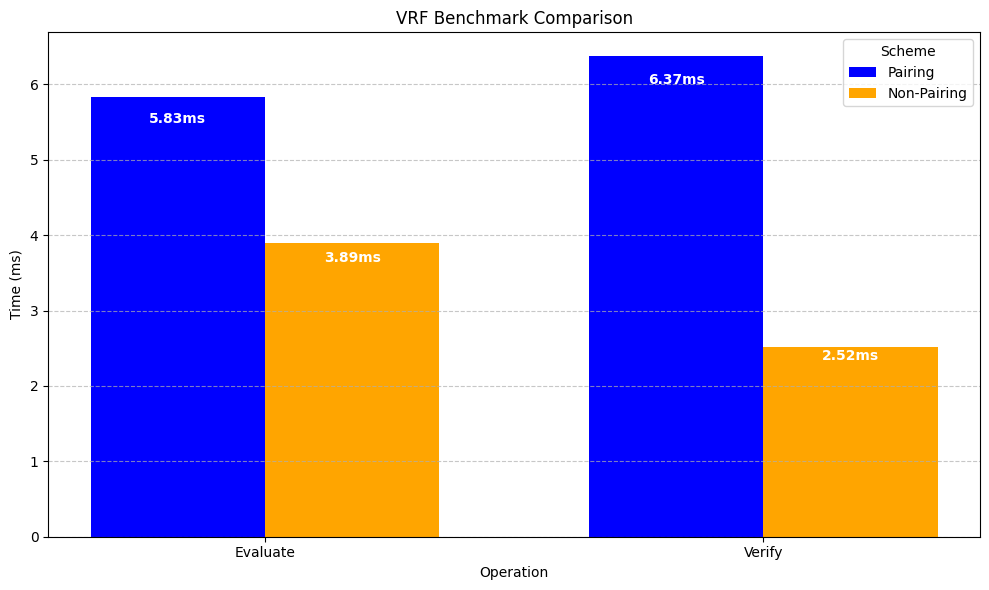
\includegraphics[width=0.75\linewidth]{figures/vrf-benchmark.png}
    \caption{VRF Benchmark}
    \label{fig:vrf-benchmark}
\end{figure}





























We first present the preliminaries and foundations of our VRF for committed inputs, the design of our $\Sigma$-protocol, and demonstrate how the integration achieves sybil resistance in anonymous credential systems.

\begin{definition}[Sybil-Resistant Issuance]
For any context $\ctx$, a Context Credential issuer must be able to detect if a user with master credential containing identifier $\id$ has previously obtained a context credential for $\ctx$, without learning $\id$ itself or linking this issuance request to other credential presentations.
\end{definition}

\[
\cmm = \mathsf{CM.Com}([\id, \k, \ctx, \exp]; r) = g_1^{\id}, g_2^{\k}, g_3^{\ctx}, g_4^{\exp} g^r \quad \wedge \quad \cmc = \mathsf{CM.Com}([\id, \ctx, \exp]; r_2) = g_1^{\id}g_2^{\ctx}g^{r_2}
\]
During Context Credential issuance, a user must prove to the issuer that their context credential hasn't been issued before, that is, the Context Credential issuance must be \emph{Sybil Resistant}. Our goal is to generate a unique, unlinkable nullifier for a specific context containing something in both the Master Credential and the Context Credential to protect the system from Sybil attacks while also retaining user privacy.

We leverage the structure and properties of the Dodis Yampolisky Verifiable Random Function (VRF)
\[
\text{Nullifier } \textsf{N} = g^{1/k + \textsf{ctx}}
\]

The Nullifier takes on the properties of correctness, pseudorandomness, and provable uniqueness from the VRF which we exploit in our protocol.




\subsection{Algebraic Analysis of Dodis Yampolskiy VRF}
We first recall the classical Dodis Yampolskiy VRF construction with bilinear pairings, we demonstrate with Type-3 pairings as they are generally used in practice. Let $\G_1, \G_2, \G_T$ be groups of a bilinear map with prime order $p$ where $g_1, g_2$ are generators for $\G_1, \G_2$ respectively and $e$ is an efficient map from $\G_1 \times \G_2 \to \G_T$:

% \begin{itemize}
%     \item $\mathsf{VRF.Gen}(\secparam)$: Samples $k \sample \Z_p$, set $pk = g^k$ 
    
%     \item $\mathsf{VRF.Eval}(k, \ctx) \to $(\mathsf{N}, \pi)$: $\pi = e(g_1, g_2)^{1/(k + \textsf{ctx})}$, $\mathsf{N} = g_2^{1/(k + \textsf{ctx})}$ 
    
%     \item $\mathsf{VRF.Vfy}(pk, \textsf{ctx}, \mathsf{N}, \pi) \to \bit$: assert $\quad$ $e(g^{\textsf{ctx}} \cdot pk, \mathsf{N})  \stackrel{?}{=} e(g_1, g_2) \quad \wedge \quad \pi  \stackrel{?}{=} e(g_1, \mathsf{N})$
% \end{itemize}

$\mathsf{Eval}$ computes the nullifier $\textsf{N}$ and generates a proof $\pi$ to prove that anyone in possession of $pk$ and the input $\textsf{ctx}$ can verify $\textsf{N}$ was computed correctly. $\mathsf{Vfy}$ resembles a signature verification as it binds  the public key $pk$, input $\textsf{ctx}$, and nullifier output together. 

The first pairing binds the public input $pk, \mathsf{ctx}$ with $\mathsf{N}$
\begin{align*}
    e(g_1^\mathsf{ctx} \cdot pk, \mathsf{N})  \quad  \stackrel{?}{=}& \quad  e(g_1, g_2) \\
    e(g_1^\mathsf{ctx}, g_2^{1/(k + \mathsf{ctx})}) \cdot  e(pk, g_2^{1/(k + \mathsf{ctx})}) \quad  \stackrel{?}{=}& \quad  e(g_1, g_2) \\
    e(g_1^\mathsf{ctx}, g_2)^{1/(k + \mathsf{ctx})} \cdot  e(g_1^k, g_2)^{1/(k + \mathsf{ctx})} \quad  \stackrel{?}{=}& \quad  e(g_1, g_2) \\
    e(g_1, g_2)^{\mathsf{ctx}/(k + \mathsf{ctx})} \cdot  e(g_1^k, g_2)^{k/(k + \mathsf{ctx})} \quad  \stackrel{?}{=}& \quad  e(g_1, g_2) \\
    e(g_1, g_2)^{\mathsf{ctx} + k/(k + \mathsf{ctx})}  \quad =& \quad e(g_1, g_2) \\
\end{align*}

\begin{align*}
     \pi  \quad  \stackrel{?}{=}& \quad e(g_1, \mathsf{N}) \\
     e(g_1, g_2)^{1/(k + \textsf{ctx})}  \stackrel{?}{=}& \quad  e(g_1, g_2^{1/(k + \mathsf{ctx})}) \\
     e(g_1, g_2)^{1/(k + \textsf{ctx})}  \stackrel{?}{=}& \quad  e(g_1, g_2)^{1/(k + \textsf{ctx})} \\
\end{align*}

% And the second pairing binds the proof $\pi$ to \mathsf{N}$

\subsubsection{Informal Security analysis of Bilinear Pairing VRF}
\begin{itemize}
    \item \textbf{Correctness:} Follows directly from pairing properties. The algebraic structure ensures verification equations hold when computed honestly.
    
    \item \textbf{Unique Provability:} Each nullifier $\mathsf{N} = g_2^{1/(k+\textsf{ctx})}$ is uniquely determined by the pairing equation $e(g_1^{k + \textsf{ctx}}, \mathsf{N}) = e(g_1, g_2)$. A forgery requires solving DLOG to create  $g_2^{1/(k+\textsf{ctx}')} = \mathsf{N}$.
    
    \item \textbf{Pseudorandomness:} Relies on the $q$-DHI assumption in bilinear groups. Given $g_1, g_1^k, g_1^{k^2}, \ldots$, distinguishing $\mathsf{N} = g_2^{1/(k+\textsf{ctx})}$ from random reduces to computing $g_2^{1/k}$ (a $q$-DHI instance).
\end{itemize}



\subsection{VRF with Committed Inputs}
As demonstrated above, the classical Dodis-Yampolskiy VRF uses pairings to verify the relationship between inputs and outputs through the equation: $e(g_1^{\textsf{ctx}} \cdot pk, \mathsf{N}) = e(g_1, g_2)$. Our key insight is that this pairing equation fundamentally verifies a multiplicative relationship $(k + \textsf{ctx}) \cdot \frac{1}{k + \textsf{ctx}} = 1$:

\begin{align*}
    e(g_1^{\textsf{ctx}} \cdot pk, \mathsf{N}) =& e(g_1, g_2)    \\
    e(g_1^{\textsf{ctx}} \cdot g_1^k, g_2^{1/(k + \textsf{ctx})}) =& e(g_1, g_2) \\
    e(g_1^{\textsf{ctx + k}}, g_2^{1/(k + \textsf{ctx})}) =& e(g_1, g_2) \\
    (\textsf{ctx + k}) \cdot 1/(k + \textsf{ctx})  =& 1 \\
\end{align*}

% This observation suggests an alternative approach: instead of using pairings to verify this relationship, we can prove it directly through a carefully constructed $\Sigma$-protocol. Let:
% \begin{itemize}
%     \item $m_1 = k + \textsf{ctx}$ (committed in $\cm_1$)
%     \item $m_2 = \frac{1}{k + \textsf{ctx}}$ (committed in $\cm_2$)
% \end{itemize}

% The VRF nullifier is then simply $\mathsf{N} = g^{m_2}$, and verification reduces to proving:
% \begin{enumerate}
%     \item $m_1$ is correctly formed from committed values $k$ and $\textsf{ctx}$
%     \item $m_1 \cdot m_2 = 1$ (multiplicative inverse relation)
%     \item $\mathsf{N} = g^{m_2}$ (nullifier structure)
% \end{enumerate}

% This reformulation eliminates the need for pairings while maintaining the security properties of the original VRF. The challenge now becomes constructing an efficient $\Sigma$-protocol that proves these relationships without revealing the underlying values.



% \subsection{Commitment Structure for VRF Verification}
% To privately prove the VRF relationship, we commit to both the input relationship and multiplicative inverse:

% % \begin{itemize}
% %     \item Primary commitments to inputs:
% %         \[\cm_k = g^k h^{r_1}, \quad \cm_{\textsf{ctx}} = g^{\textsf{ctx}} h^{r_2}\]
    
% %     \item Derived commitment to their sum:
% %         \[\cm_3 = \cm_k^{\textsf{ctx}} h^{r_3}
    
% %     \item Commitment to the inverse:
% %         \[\cm_4 = \cm^{m_2} h^{r_4} \text{ where } m_2 = \frac{1}{m_1}\]
% % \end{itemize}

% The algebraic structure of these commitments enables our $\Sigma$-protocol to efficiently prove the multiplicative inverse relationship while maintaining zero-knowledge.


% \subsection{Sigma-Protocol Construction}
% Given these commitments, we construct a $\Sigma$-protocol that proves the VRF relationship in zero-knowledge. The protocol leverages auxiliary commitments $\cm_3, \cm_4$
% to enforce the multiplicative inverse relationship: $\Pi^{\mathcal{R}_{\textsf{VRF}}}$ from 

%     \[
%         \mathcal{R}_{\mathsf{vrf}} = \left\{ (\cm_k, \cm_{\textsf{ctx}}, \mathsf{N}), (k, \textsf{ctx}, r_1, r_2) \; \Big| \;  \cm_k = g^k h^{r_1} \; \land \;
%                 \cm_{\textsf{ctx}} = g^{\textsf{ctx}} h^{r_2} \land \textsf{N} = g^{1/(k + \textsf{ctx})} \right\}
%     \]


\newpage
\begin{protocol}{Non-Pairing VRF Output Verification}{non-pairing-vrf-verify}\label{pok-non-pairing-vrf}
\textbf{Common Input:} Group generators $g_1, g_2, g_3, g_4, g_5, g \in \mathbb{G}$, and commitments $\cm_1, \cm_2, \cm_3, \cm_4, \cm_5, \cm_6 \in \mathbb{G}$\\
\textbf{Prover Input:} Witness $(\id, \k, \ctx, r_1, r_2, r_3, r_4, r_5, \textsf{n}, r_6)$ such that:
    \begin{align*}
        \cm_1 &= g_1^{\id} g_2^{\k} g^{r_1}     &    \cm_2 &= g_1^{\id} g_3^{\ctx} g^{r_2}  &   \cm_3 &= g_4^{\k + \ctx} g^{r_3}\\
        \cm_4 &= g_5^{\textsf{n}} g^{r_4}   &   \cm_5 &= \cm_3^{\textsf{n}} g^{r_5}     &   \cm_6 &= g^{r_6} \\
        \textsf{n} &= \frac{1}{\k + \ctx}   &   r_6 &= r_3 \cdot \textsf{n} + r_5    &   \frac{\cm_5}{\cm_6} &= g_4 \\
    \end{align*}

\begin{enumerate}
    \item \textbf{Commitment:} Prover samples random blinding factors from $\Z_q$:
    \[
        a_x \quad \text{ for } \quad x \in \{\ \id, \k, \ctx, \textsf{n}, r_1, \ldots,r_6\} \in \Z_q
    \]
    \textbf{Computes}:
    \begin{align*}
        T_1 &\gets g_1^{a_{\id}} g_2^{a_k} g^{a_{r_1}}  &   T_2 &\gets g_1^{a_{\id}} g_3^{a_{\ctx}} g^{a_{r_2}}     &   T_3 &\gets g_4^{a_k + a_{\ctx}} g^{a_{r_3}} \\
        T_4 &\gets g_5^{a_{\textsf{n}}} g^{a_{r_4}}   &   T_5 &\gets \cm_3^{a_{\textsf{n}}} g^{a_{r_5}}     &   T_6 &\gets g^{a_{r_6}}
    \end{align*}
    Sends $(T_1, T_2, T_3, T_4, T_5, T_6)$ to verifier.
    
    \item \textbf{Challenge:} Verifier samples $c \sample \mathbb{Z}_q$ and sends to prover.
    
    \item \textbf{Response:} Prover computes:
    \[
    z_x = a_x + c \cdot x \quad \text{ for } \quad x \in \{\ \id, \k, \ctx, \textsf{n}, r_1, \ldots,r_6\} 
    \]
    Sends $(z_{\id}, z_k, z_{\ctx}, z_{r_1}, z_{r_2}, z_{r_3}, z_{\textsf{n}}, z_{r_4}, z_{r_5}, z_{r_6})$ to verifier.
    
    \item \textbf{Verification:} Verifier checks:
    \begin{enumerate}[label=(\roman*)]
        \item $g_1^{z_{\id}} g_2^{z_k} g^{z_{r_1}} \stackrel{?}{=} T_1 \cdot \cm_1^c$
        \item $g_1^{z_{\id}} g_3^{z_{\ctx}} g^{z_{r_2}} \stackrel{?}{=} T_2 \cdot \cm_2^c$
        \item $g_4^{z_k + z_{\ctx}} g^{z_{r_3}} \stackrel{?}{=} T_3 \cdot \cm_3^c$
        \item $g_5^{z_{\textsf{n}}} g^{z_{r_4}} \stackrel{?}{=} T_4 \cdot \cm_4^c$
        \item $\cm_3^{z_{\textsf{n}}} g^{z_{r_5}} \stackrel{?}{=} T_5 \cdot \cm_5^c$
        \item $g^{z_{r_6}} \stackrel{?}{=} T_6 \cdot \cm_6^c$
        \item $\frac{\cm_5}{\cm_6} \stackrel{?}{=} g_4$
    \end{enumerate}
\end{enumerate}
\end{protocol}








\newpage
\paragraph{Security Analysis:}
The protocol satisfies the following security properties:

\begin{itemize}
    \item \textbf{Completeness:} For an honest prover and verifier, all verification equations hold algebraically:
\begin{align*}
        g_1^{z_{\id}} g_2^{z_k} g^{z_{r_1}} &= g_1^{a_{\id} + c \cdot \id} g_2^{a_k + c \cdot \k} g^{a_{r_1} + c \cdot r_1} = T_1 \cdot \cm_1^c \\
        g_1^{z_{\id}} g_3^{z_{\ctx}} g^{z_{r_2}} &= g_1^{a_{\id} + c \cdot \id} g_3^{a_{\ctx} + c \cdot \ctx} g^{a_{r_2} + c \cdot r_2} = T_2 \cdot \cm_2^c \\
        g_4^{z_k + z_{\ctx}} g^{z_{r_3}} &= g_4^{(a_k + c \cdot \k) + (a_{\ctx} + c \cdot \ctx)} g^{a_{r_3} + c \cdot r_3} = T_3 \cdot \cm_3^c \\
        g_5^{z_{\textsf{n}}} g^{z_{r_4}} &= g_5^{a_{\textsf{n}} + c \cdot \textsf{n}} g^{a_{r_4} + c \cdot r_4} = T_4 \cdot \cm_4^c \\
        \cm_3^{z_{\textsf{n}}} g^{z_{r_5}} &= \cm_3^{a_{\textsf{n}} + c \cdot \textsf{n}} g^{a_{r_5} + c \cdot r_5} = T_5 \cdot \cm_5^c \\
        g^{z_{r_6}} &= g^{a_{r_6} + c \cdot r_6} = T_6 \cdot \cm_6^c \\
        \frac{\cm_5}{\cm_6} &= g_4^{(\k + \ctx) \cdot \textsf{n}} = g_4 \quad \text{since} \quad (\k + \ctx) \cdot \textsf{n} = 1
    \end{align*}
    
    \item \textbf{Special Soundness:} Given two accepting transcripts $(T_1, T_2, T_3, T_4, T_5, T_6, c, z_{\id}, z_k, z_{\ctx}, z_{r_1}, z_{r_2}, z_{r_3}, z_{\textsf{n}}, z_{r_4}, z_{r_5}, z_{r_6})$ and $(T_1, T_2, T_3, T_4, T_5, T_6, c', z_{\id}', z_k', z_{\ctx}', z_{r_1}', z_{r_2}', z_{r_3}', z_{\textsf{n}}', z_{r_4}', z_{r_5}', z_{r_6}')$ with $c \neq c'$, the extractor $\mathcal{E}$ computes:
    \begin{align*}
        \id &= \frac{z_{\id} - z_{\id}'}{c - c'} & \k &= \frac{z_k - z_k'}{c - c'} & \ctx &= \frac{z_{\ctx} - z_{\ctx}'}{c - c'} \\
        r_1 &= \frac{z_{r_1} - z_{r_1}'}{c - c'} & r_2 &= \frac{z_{r_2} - z_{r_2}'}{c - c'} & r_3 &= \frac{z_{r_3} - z_{r_3}'}{c - c'} \\
        \textsf{n} &= \frac{z_{\textsf{n}} - z_{\textsf{n}}'}{c - c'} & r_4 &= \frac{z_{r_4} - z_{r_4}'}{c - c'} & r_5 &= \frac{z_{r_5} - z_{r_5}'}{c - c'} & r_6 &= \frac{z_{r_6} - z_{r_6}'}{c - c'}
    \end{align*}
    The extracted witness satisfies all commitment relations and the multiplicative inverse $\textsf{n} = \frac{1}{\k + \ctx}$ due to the binding property of Pedersen commitments.
    
    \item \textbf{Honest-Verifier Zero-Knowledge:} The simulator $\mathcal{S}$ operates as follows:
    \begin{enumerate}
        \item Sample $z_{\id}, z_k, z_{\ctx}, z_{r_1}, z_{r_2}, z_{r_3}, z_{\textsf{n}}, z_{r_4}, z_{r_5}, z_{r_6} \sample \mathbb{Z}_q$ uniformly.
        \item Compute simulated commitments:
        \begin{align*}
            T_1 &\gets g_1^{z_{\id}} g_2^{z_k} g^{z_{r_1}} \cdot \cm_1^{-c} \\
            T_2 &\gets g_1^{z_{\id}} g_3^{z_{\ctx}} g^{z_{r_2}} \cdot \cm_2^{-c} \\
            T_3 &\gets g_4^{z_k + z_{\ctx}} g^{z_{r_3}} \cdot \cm_3^{-c} \\
            T_4 &\gets g_5^{z_{\textsf{n}}} g^{z_{r_4}} \cdot \cm_4^{-c} \\
            T_5 &\gets \cm_3^{z_{\textsf{n}}} g^{z_{r_5}} \cdot \cm_5^{-c} \\
            T_6 &\gets g^{z_{r_6}} \cdot \cm_6^{-c}
        \end{align*}
        \item Output $(T_1, T_2, T_3, T_4, T_5, T_6, c, z_{\id}, z_k, z_{\ctx}, z_{r_1}, z_{r_2}, z_{r_3}, z_{\textsf{n}}, z_{r_4}, z_{r_5}, z_{r_6})$.
    \end{enumerate}
    The simulated transcript is perfectly indistinguishable from a real transcript since the $z$-values are uniformly random and the $T_i$ are uniquely determined by the verification equations.
\end{itemize}

\paragraph{Connection to VRF Security}
The protocol’s soundness ensures that $\textsf{n} = \frac{1}{\k + \ctx}$ is correctly computed and tied to the commitments, critical for:
\begin{itemize}
    \item \textbf{Pseudorandomness:} Under the $q$-DHI assumption, $\textsf{n}$ is indistinguishable from random without knowing $\k$.
    \item \textbf{Uniqueness:} The relation $\frac{\cm_5}{\cm_6} = g_4$ enforces $(\k + \ctx) \cdot \textsf{n} = 1$, ensuring a unique nullifier per $(\k, \ctx)$ pair.
\end{itemize}
Thus, the VRF’s security reduces to the discrete logarithm assumption and the soundness of the inverse proof.






















































































\paragraph{Security Analysis:}
The protocol satisfies the following security properties:

\begin{itemize}
    \item \textbf{Completeness:} For honest prover and verifier, all verification equations hold algebraically:
    \begin{align*}
        g^{s_1}h^{u_1} &= g^{\alpha_1 + cm_1}h^{\rho_1 + cr_1} = T_1 \cdot \cm_1^c\\
        g^{s_2}h^{u_2} &= g^{\alpha_2 + cm_2}h^{\rho_2 + cr_2} = T_2 \cdot \cm_2^c\\
        \cm_1^{s_2}h^{u_3} &= \cm_1^{\alpha_2 + cm_2}h^{\rho_3 + cr_3} = T_3 \cdot \cm_3^c\\
        h^{u_4} &= h^{\rho_4 + cr_4} = T_4 \cdot \cm_4^c
    \end{align*}
    
    \item \textbf{Special Soundness:} Given two accepting transcripts $(T_1, T_2, T_3, T_4, c, s_1, s_2, u_1, u_2, u_3, u_4)$ and $(T_1, T_2, T_3, T_4, c', s_1', s_2', u_1', u_2', u_3', u_4')$ with $c \neq c'$, the extractor $\mathcal{E}$ works as follows:
    \begin{align*}
        m_1 &= \frac{s_1 - s_1'}{c - c'} &r_1 &= \frac{u_1 - u_1'}{c - c'}\\
        m_2 &= \frac{s_2 - s_2'}{c - c'} &r_2 &= \frac{u_2 - u_2'}{c - c'}\\
        r_3 &= \frac{u_3 - u_3'}{c - c'} &r_4 &= \frac{u_4 - u_4'}{c - c'}
    \end{align*}
    The extracted witness satisfies all verification equations and the multiplicative inverse relation by the binding property of Pedersen commitments.
    
    \item \textbf{Honest-Verifier Zero-Knowledge:} The simulator $\mathcal{S}$ operates as follows:
    \begin{enumerate}
        \item Sample $s_1, s_2, u_1, u_2, u_3, u_4 \sample \Z_q$ uniformly
        \item Compute simulated commitments:
        \begin{align*}
            T_1 &\gets g^{s_1}h^{u_1} \cdot \cm_1^{-c}\\
            T_2 &\gets g^{s_2}h^{u_2} \cdot \cm_2^{-c}\\
            T_3 &\gets \cm_1^{s_2}h^{u_3} \cdot \cm_3^{-c}\\
            T_4 &\gets h^{u_4} \cdot \cm_4^{-c}
        \end{align*}
        \item Output $(T_1, T_2, T_3, T_4, c, s_1, s_2, u_1, u_2, u_3, u_4)$
    \end{enumerate}
    The simulated transcript is perfectly indistinguishable from a real transcript as the distribution of responses $(s_1, s_2, u_1, u_2, u_3, u_4)$ is uniform in both cases, and the commitments are uniquely determined by the verification equations.
\end{itemize}

\paragraph{Connection to VRF Security}  
The protocol’s soundness guarantees that $\textsf{N} = g^{m_2}$ is valid only if $m_2 = 1/m_1$ for $m_1 = k + \textsf{ctx}$. This is critical because:
\begin{itemize}
    \item \textbf{Pseudorandomness:} Under $q$-DHI, $g^{1/m_1}$ is indistinguishable from random without knowledge of $m_1$.
    \item \textbf{Uniqueness:} The equation $m_1 \cdot m_2 = 1$ has a unique solution in $\Zp^*$, preventing adversarial equivocation.
\end{itemize}
Thus, the security of the VRF directly reduces to the hardness of computing discrete logarithms and the soundness of the inverse proof.





















\newpage

















\section{Our Contributions}

We improve the state of the art in privacy-preserving credential systems by creating a lightweight, efficient VRF construction specifically tailored for sybil resistance in anonymous credentials:

\subsection{Pairing-Free VRF in Prime-Order Groups}

We present a novel adaptation of the Dodis-Yampolskiy VRF structure that eliminates the need for computationally expensive bilinear pairings. Our construction:

\begin{itemize}
    \item Operates entirely in a single prime-order group ($\G_1$)
    \item Achieves provable pseudorandomness under the $q$-Diffie-Hellman Inversion ($q$-DHI) assumption
    \item Produces verifiable nullifiers of the form $\nul = g^{1/(k+\text{ctx})}$ where $k$ is a credential-specific secret and $\text{ctx}$ is the context identifier
\end{itemize}

This adaptation significantly reduces computational overhead compared to pairing-based alternatives while maintaining the same security guarantees.

\subsection{Zero-Knowledge Proof of Multiplicative Inverse}

We introduce an efficient $\Sigma$-protocol that proves the relationship between committed values $m_1 = k+\text{ctx}$ and $m_2 = 1/m_1$ without revealing either value. This protocol:

\begin{itemize}
    \item Enables verification of VRF outputs without compromising credential privacy
    \item Uses auxiliary commitments to enforce the multiplicative inverse relation
    \item Achieves perfect honest-verifier zero-knowledge
    \item Generalizes naturally to other cryptographic scenarios requiring proofs of inverse relationships
\end{itemize}

Our protocol structure can be applied beyond VRFs to any system requiring proofs of multiplicative inverse relationships in zero-knowledge.

\subsection{Formal Security Guarantees}

We demonstrate that sybil resistance in our system reduces to:
\begin{itemize}
    \item The $q$-DHI assumption in prime-order groups
    \item The binding property of Pedersen commitments
    \item The soundness of our $\Sigma$-protocol
\end{itemize}

These formal security guarantees ensure our construction maintains:
\begin{itemize}
    \item \textbf{Pseudorandomness:} VRF outputs are indistinguishable from random without knowledge of the secret
    \item \textbf{Uniqueness:} One nullifier per $(k,\text{ctx})$ pair, preventing sybil attacks
    \item \textbf{Unlinkability:} Multiple uses of the same credential remain unlinkable
\end{itemize}

\subsection{Efficiency Improvements}

Our experimental evaluation demonstrates substantial performance gains over pairing-based approaches:
\begin{itemize}
    \item 33\% faster evaluation (3.89ms vs. 5.83ms)
    \item 60\% faster verification (2.52ms vs. 6.37ms)
\end{itemize}

These improvements directly translate to enhanced scalability and user experience in credential systems, particularly on resource-constrained devices where bilinear pairings are prohibitively expensive.












\newpage
\section{Technical Construction}

We now present our pairing-free VRF construction, starting with essential preliminaries and then detailing our protocol for creating and verifying nullifiers in zero-knowledge.

\subsection{Preliminaries}

\begin{definition}[$q$-DHI Assumption]
Let $\mathbb{G}$ be a cyclic group of prime order $p$ with generator $g$. The $q$-Diffie-Hellman Inversion ($q$-DHI) assumption states that for any PPT adversary $\mathcal{A}$, there exists a negligible function $\mathsf{negl}$ such that:
\[
\Pr\left[x \leftarrow \mathbb{Z}_p^*, \mathcal{A}(g, g^x, g^{x^2}, \ldots, g^{x^q}) = g^{1/x}\right] \leq \mathsf{negl}(\lambda)
\]
\end{definition}

\begin{remark}
The $q$-DHI assumption is equivalent to the $(q+1)$-generalized Diffie-Hellman assumption as shown by Boneh and Boyen \cite{BB04}. This equivalence provides a solid theoretical foundation for our VRF construction's security.
\end{remark}

\begin{definition}[Verifiable Random Function in Prime-Order Group]
A VRF in a prime-order group $\mathbb{G}$ is a tuple of algorithms $(\mathsf{VRF.Gen}, \mathsf{VRF.Eval}, \mathsf{VRF.Vfy})$ with message space $\mathcal{X}$, output space $\mathcal{Y}$, and proof space $\Pi$ satisfying:

\begin{itemize}
    \item $\mathsf{VRF.Gen}(1^\lambda) \rightarrow (sk, pk)$: Samples secret key $sk \leftarrow \mathbb{Z}_p^*$, computes public key $pk = g^{sk}$
    \item $\mathsf{VRF.Eval}(sk, x) \rightarrow (y, \pi)$: Computes output $y = g^{1/(sk+x)}$ and proof $\pi$
    \item $\mathsf{VRF.Vfy}(pk, x, y, \pi) \rightarrow \{0,1\}$: Verifies that $y = g^{1/(sk+x)}$
\end{itemize}

with correctness, unique provability, and pseudorandomness properties as defined in standard VRF literature.
\end{definition}

\subsection{From Pairing-Based to Pairing-Free VRF}

We begin by analyzing the classic Dodis-Yampolskiy VRF, which relies on bilinear pairings. In this construction, verification proceeds by checking:
\[
e(g_1^{\text{ctx}} \cdot pk, N) \stackrel{?}{=} e(g_1, g_2)
\]

where $N = g_2^{1/(k+\text{ctx})}$ is the VRF output, $pk = g_1^k$ is the public key, and $e: \mathbb{G}_1 \times \mathbb{G}_2 \rightarrow \mathbb{G}_T$ is a bilinear pairing.

Expanding this equation:
\[
e(g_1^{\text{ctx}} \cdot g_1^k, g_2^{1/(k+\text{ctx})}) = e(g_1, g_2)
\]

This verification essentially proves that $(k+\text{ctx}) \cdot \frac{1}{k+\text{ctx}} = 1$.

Our key insight is that we can eliminate the pairing by directly proving this multiplicative inverse relationship. We define:
\begin{align}
m_1 &= k + \text{ctx} \\
m_2 &= \frac{1}{k+\text{ctx}}
\end{align}

With these values, the nullifier becomes $N = g^{m_2}$, and verification reduces to proving that $m_1 \cdot m_2 = 1$.

\subsection{Commitment Structure for VRF Verification}

To support zero-knowledge proofs of the VRF relationship, we use the following commitment structure:

\begin{align}
\text{cm}_1 &= g_1^{\text{id}} \cdot g_2^{k} \cdot g^{r_1} \\
\text{cm}_2 &= g_1^{\text{id}} \cdot g_3^{\text{ctx}} \cdot g^{r_2} \\
\text{cm}_3 &= g_4^{\text{exponent\_k\_ctx}} \cdot g^{r_3} \\
\text{cm}_4 &= g_5^{\text{exponent\_k\_ctx\_inv}} \cdot g^{r_4} \\
\text{cm}_5 &= \text{cm}_3^{\text{exponent\_k\_ctx\_inv}} \cdot g^{r_5} \\
\text{cm}_6 &= g^{r_6}
\end{align}

where $\text{exponent\_k\_ctx} = k + \text{ctx}$ and $\text{exponent\_k\_ctx\_inv} = 1/\text{exponent\_k\_ctx}$.

This commitment structure allows us to prove:
\begin{enumerate}
    \item $\text{cm}_1$ and $\text{cm}_2$ contain the same id
    \item $\text{cm}_3$ contains the sum of $k$ and ctx from $\text{cm}_1$ and $\text{cm}_2$
    \item $\text{cm}_4$ contains the inverse of the value in $\text{cm}_3$
    \item $\text{cm}_3 \cdot \text{cm}_4$ equals the identity element (proving the inverse relationship)
    \item The nullifier $N = g_4$ is correctly formed
\end{enumerate}


































\subsection{Technical Construction}

Preliminaries: q-DHI assumption, VRF definition
Our Construction:

From pairing-based to pairing-free VRF
Commitment structure for verification
Complete sigma-protocol description (aligned with your code)


Security Analysis: Sketch of completeness, soundness, zero-knowledge







4. Performance Evaluation (1/2 page)

Benchmark methodology
Results comparison with pairing-based approach
Interpretation of performance gains for credential systems
























In the $\MIMCABC$ system, identity binding ensures all credentials in a presentation belong to the same user by proving the equality of a committed identifier $\id$ across credentials. This enables users to prove multiple credentials together for application scenarios.
Credential Relationship binding extends this, enabling users to prove structured relationships between anonymous credentials, such as generating single-use tokens for integration with other systems e.g. privacy-pass-like applications \cite{davidson2018privacy} and for sybil-resistant context credentials.

Identity binding links credentials to a single user identifier, credential relationship binding enforces dependency constraints between credentials, and a credential relationship bound nullifier is a deterministic anonymous token that proves the user has this relationship. Because it's determinisitic and based on the users secret attributes, they can only derive it in the same way, so the token is used for Sybil Resistance scenarios where privacy is still required and furthermore can be used in Revocation checks.

Sybil Resistance in private systems is difficult and furthermore in a multi-issuer, multi-credential scenario, simple relationship binding is not enough, as in $\MIMCABC$ a user can more easily maliciously create credentials with lower-security issuers that allow them to prove identity binding with attributes of their choice. 

\subsection{Limitation of existing approaches}
\begin{enumerate}
    \item \textbf{Standard VRF} verifies a nullifier $\nul$ by computes a deterministic nullifier
    \[
        \nul \gets g^{1/(\key + \ctx)}    \qquad \nul \cdot (\pk)^{\ctx}
    \]
    
    where $\key$ is the secret key, $\pk = g^{\key}$ is the public key, and $\nul$ is verifiable by $\nul \cdot (\pk)^{\ctx}$ for a public $\ctx$. This does not preserve the anonymity notions required for Anonymous Credentials as $\pk$ is publicly used each usage
    
    \item \textbf{MPC PRF}: CanDID, a decentralized identity system, computes nullifiers from MPC PRF during credential issuance preserving anonymity properties with secure multiparty computation, which has large overhead, and because of the time spent during PRF generation, can't be used easily for other mechanisms like the output being in a revocation list.
    
    \item \textbf{Pairing-based VRF:}  We base our scheme on the notions in \cite{tomescu2022utt}, our novel contribution is its computation in $\G_1$ and thus removing the pairing computation and operation in $\G_2$, improving computation efficiency and allowing its use in non-pairing based schemes.
\end{enumerate}

\subsection{Credential Relationship Bound Verifier from Pairing-Free VRF}
\begin{itemize}
    \item VRF Overview: A Verifiable Random Function generates a pseudorandom, deterministic output nullifier 
    \[
    \nul \gets g^{1/(\key + \ctx)}
    \]
    Verifiable by a public key $\pk = g^{\key}$. In $\MIMCABC, \key$ is a committed attribute in a master credential and $\ctx$ is the unique identifier of the context credential

    \item Integration: Users commit $\key$ and $\ctx$ in Pedersen commitments e.g., $( \cm_k = g^{\key} h^r, \cm_{\ctx} = g^{\ctx} h^{r_2})$, compute the nullifier, and prove its correctness to the issuer using a zero-knowledge protocol. This ensures one nullifier per $(\key, \ctx)$ pair, preventing sybil attacks.
\end{itemize}

\subsection{Contributions}

\noindent We improve the state of the art by creating a lightweight VRF construction tailored for Anonymous Credential systems with 3 contributions:
\begin{enumerate}
        \item \textbf{Pairing-Free VRF in Prime-Order Groups:} We adapt the Dodis-Yampolskiy VRF structure to function efficiently in standard prime-order groups, achieving provable pseudorandomness under the $q$-Diffie-Hellman Inversion ($q$-DHI) assumption.

        \item \textbf{Zero-Knowledge Proof of Multiplicative Inverse:} We introduce a novel $\Sigma$-protocol that proves the multiplicative inverse relation between committed values $m_1 = k + \textsf{ctx}$ and $m_2 = 1/m_1$, we use it in our scheme to verify the correctness of the VRF nullifier without revealing user secrets. We show it generalizes naturally for similar requirements in $\Sigma$-protocols, especially those needing to prove the q-DHI.

         \item \textbf{Formal Security Guarantees:} We demonstrate sybil resistance reduces to the security of our construction, the unique provability of the vrf and the soundness of our $\Sigma$-protocol.
\end{enumerate}

\newpage
\section{Extra}




















\subsection{Preliminaries}

\begin{definition}[q-DHI Assumption]
Let $\mathbb{G}$ be a cyclic group of prime order $p$ with generator $g$. The $q$-Diffie-Hellman Inversion ($q$-DHI) assumption \cite{mitsunari_new_2002} states that for any PPT adversary $\mathcal{A}$, there exists a negligible function $\negl$ such that:
\[
\Pr\left[ x \sample \Zp^*, \quad \mathcal{A}(g, g^x, g^{x^2}, \ldots, g^{x^q}) = g^{1/x} \right] \leq \negl 
\]
where the probability is taken over the random choice of $x$ and the random coins of $\mathcal{A}$. Informally, no $\PPT$ adversary can distinguish between $g^{1/\alpha}$ from a random group element.
\end{definition}

\begin{remark}
The $q$-DHI assumption is equivalent to the $(q+1)$-generalized Diffie-Hellman assumption (GDH) as shown by Boneh and Boyen \cite{kanade_efficient_2004}. This equivalence provides a solid theoretical foundation for our VRF construction's security.
\end{remark}




\begin{definition}[Verifiable Random Function in Prime-Order Group]
A Verifiable Random Function (VRF) in prime-order group $\G$ of order $q$ is a tuple of PPT algorithms $(\mathsf{VRF.Gen}, \mathsf{VRF.Eval}, \mathsf{VRF.Vfy})$ with associated message space $\setX$, output space $\setN$, and proof space $\Pi$, defined as:

\begin{itemize}
    \item $\mathsf{VRF.Gen}(1^\lambda) \to (sk, pk):$ Samples secret key $\alpha \sample \Zp^*$, computes public key $pk \gets g^\alpha$, returns $(sk = \alpha, pk)$
    
    \item $\mathsf{VRF.Eval}(sk, x) \to \textsf{N}, \pi:$ Returns output $\textsf{N} \gets g^{1/(x+sk)}$ and $\pi$ verifies the output $\textsf{N}$
    
    \item $\mathsf{VRF.Vfy}(pk, x, \textsf{N}, \pi) \to \bit:$ validates proof $\pi$ that $\textsf{N} = g^{1/(x+sk)}$, outputs 1 for success, 0 for failure
\end{itemize}
\end{definition}

\begin{itemize}
    \item \textbf{Correctness:} For all $(sk, pk) \gets \mathsf{VRF.Gen}(1^\lambda)$ and all $x \in \setX$:
    \[
    \Pr\left[\begin{aligned}
        (y, \pi) &\gets \mathsf{VRF.Eval}(sk, x) \\
        1 &\gets \mathsf{VRF.Vfy}(pk, x, \textsf{N}, \pi)
    \end{aligned}\right] = 1
    \]

    \item \textbf{Unique Provability:} For any $pk$ (possibly malicious) and $x \in \setX$, no $\PPT$ adversary $\AdvA$ can find two distinct pairs of outputs $(\textsf{N}_0, \pi_0) \neq (\textsf{N}_1, \pi_1)$ such that:
    \[
    \mathsf{VRF.Vfy}(pk, x, \textsf{N}_0, \pi_0) = \mathsf{VRF.Vfy}(pk, x, \textsf{N}_1, \pi_1) = 1
    \]

    \item \textbf{Pseudorandomness:} For every PPT adversary $\AdvA$, there exists negligible function $\negl$ such that:
    \[
    \left|\Pr\left[\mathsf{Exp}_{\mathsf{VRF}}^{\mathsf{PR}}(\AdvA, \lambda) = 1\right] - \frac{1}{2}\right| \leq \negl
    \]
    where the pseudorandomness experiment $\mathsf{Exp}_{\mathsf{VRF}}^{\mathsf{PR}}$ is defined in the standard framework for VRFs.
\end{itemize}
